%% 
%% Copyright 2019-2024 Elsevier Ltd
%% 
%% This file is part of the 'CAS Bundle'.
%% --------------------------------------
%% 
%% It may be distributed under the conditions of the LaTeX Project Public
%% License, either version 1.3c of this license or (at your option) any
%% later version.  The latest version of this license is in
%%    http://www.latex-project.org/lppl.txt
%% and version 1.3c or later is part of all distributions of LaTeX
%% version 1999/12/01 or later.
%% 
%% The list of all files belonging to the 'CAS Bundle' is
%% given in the file `manifest.txt'.
%% 
%% Template article for cas-sc documentclass for 
%% double column output.

\documentclass[a4paper,fleqn]{cas-sc}

% If the frontmatter runs over more than one page
% use the longmktitle option.

% \documentclass[a4paper,fleqn,longmktitle]{cas-sc}

%\usepackage[numbers]{natbib}
\usepackage[numbers,sort&compress]{natbib}
\setcitestyle{maxnames=3, minnames=1}
\usepackage{bm}
\usepackage{siunitx}
\DeclareSIUnit\mmHg{mmHg}
%\usepackage[authoryear]{natbib}
% \usepackage[authoryear,longnamesfirst]{natbib}

%%%Author macros
\def\tsc#1{\csdef{#1}{\textsc{\lowercase{#1}}\xspace}}
\tsc{WGM}
\tsc{QE}
%%%

%\newcommand\revone{blue}
%\newcommand\revtwo{OliveGreen}

\newcommand\revone{black}
\newcommand\revtwo{black}

%Acrónimos
\usepackage[acronym,nomain,nonumberlist]{glossaries}
\newacronym{AAA}{AAA}{Abdominal Aorta Aneurysm}
\newacronym{AbA}{AbA}{Abdominal Aorta}
\newacronym{ACC}{ACC}{American College of Cardiology}
\newacronym{AD}{AD}{Aortic Dissection}
\newacronym{ALE}{ALE}{Arbitrary Lagrangian-Eulerian}
\newacronym{AI}{AI}{Artificial Intelligence}
\newacronym{AHA}{AHA}{American Heart Association}
\newacronym{ANN}{ANN}{Artificial Neural Networks}
\newacronym{ATA}{ATA}{Ascending Thoracic Aorta}
\newacronym{ATAA}{ATAA}{Ascending Thoracic Aortic Aneurysm}
\newacronym{AV}{AV}{Aortic Valve}
\newacronym{BAV}{BAV}{Bicuspid Aortic Valve}
\newacronym{BC}{BC}{Boundary Condition}
\newacronym{CVD}{CVD}{CardioVascular Disease}
\newacronym{CSM}{CSM}{Computational Solid Mechanics}
\newacronym{CFD}{CFD}{Computational Fluid Dynamics}
\newacronym{CT}{CT}{Computed Tomography}
\newacronym{CTA}{CTA}{Computed Tomography Angiography}
\newacronym{DL}{DL}{Deep Learning}
\newacronym{DIC}{DIC}{Digital Image Correlation}
\newacronym{DNN}{DNN}{Deep Neural Networks}
\newacronym{DNS}{DNS}{Direct Numerical Simulations}
\newacronym{DTA}{DTA}{Descending Thoracic Aorta}
\newacronym{DTAA}{DTAA}{Descending Thoracic Aortic Aneurysm}
\newacronym{ECM}{ECM}{ExtraCellular Matrix}
\newacronym{ESC}{ESC}{European Society of Cardiology}
\newacronym{FCT}{FCT}{Fundação para a Ciência e Tecnologia}
\newacronym{FDM}{FDM}{Finite Difference Method}
\newacronym{FEA}{FEA}{Finite-Element Analysis}
\newacronym{FL}{FL}{False Lumen}
\newacronym{FEM}{FEM}{Finite-Element Method}
\newacronym{FIESTA}{FIESTA}{Fast Imaging Employing Steady-state Acquisition}
\newacronym{FSI}{FSI}{Fluid-Structure Interaction}
\newacronym{FVM}{FVM}{Finite Volume Method}
\newacronym{GPU}{GPU}{Graphical Processing Unit}
\newacronym{ICP}{ICP}{Iterative Closest Point}
\newacronym{LES}{LES}{Large Eddy Simulations}
\newacronym{ML}{ML}{Machine Learning}
\newacronym{MLU}{MLU}{Media Lamellar Units}
\newacronym{MMP}{MMP}{Matrix MetalloProteinase}
\newacronym{MRI}{MRI}{Magnetic Resonance Imaging}
\newacronym{OSI}{OSI}{Oscillatory Shear Index}
\newacronym{PCA}{PCA}{Principal Component Analysis}
\newacronym{PG}{PG}{ProteoGlycan}
\newacronym{PRISMA}{PRISMA}{Preferred Reporting Items for Systematic Reviews and Meta-Analyses}
\newacronym{PT}{PT}{Prestress Tensor}
\newacronym{PWV}{PWV}{Pulse Wave Velocity}
\newacronym{PWS}{PWS}{Peak Wall Stress}
\newacronym{RANS}{RANS}{Reynolds-Averaged Navier-Stokes}
\newacronym{RLBM}{RLBM}{Regularized Lattice Boltzman Method}
\newacronym{ROM}{ROM}{Reduced Order Model}
\newacronym{RPIM}{RPIM}{Radial Point Interpolation Method}
\newacronym{SP}{SP}{Source Points}
\newacronym{SPH}{SPH}{Smoothed Particle Hydrodynamics}
\newacronym{SSM}{SSM}{Statistical Shape Model}
\newacronym{STJ}{STJ}{Sinotubular Junction}
\newacronym{RRT}{RRT}{Relative Residence Time}
\newacronym{TAA}{TAA}{Thoracic Aorta Aneurysm}
\newacronym{TAV}{TAV}{Tricuspid Aortic Valve} 
\newacronym{TAWSS}{TAWSS}{Time-Averaged Wall Shear Stress}
\newacronym{TL}{TL}{True Lumen}
\newacronym{VFM}{VFM}{Virtual Flux Method}
\newacronym{VSMC}{VSMC}{Vascular Smooth Muscle Cell}
\newacronym{XFEM}{XFEM}{Extended Finite Element Method}
\newacronym{WHO}{WHO}{World Health Organization}
\newacronym{WSS}{WSS}{Wall Shear Stress}
\newacronym{WS}{WS}{Wall Stress}
\newacronym{ZPG}{ZPG}{Zero Pressure Geometry}
%%%%%

\newcommand\invivo{\textit{in vivo}~}
% Uncomment and use as if needed
%\newtheorem{theorem}{Theorem}
%\newtheorem{lemma}[theorem]{Lemma}
%\newdefinition{rmk}{Remark}
%\newproof{pf}{Proof}
%\newproof{pot}{Proof of Theorem \ref{thm}}

%Alterar imagens sólido (SCATTER PLOTS MAINLY)
%cORRIGIR RESULTADOS

\begin{document}
\let\WriteBookmarks\relax
\def\floatpagepagefraction{1}
\def\textpagefraction{.001}

% Short title
\shorttitle{Coupling Finite Element based Models and Machine Learning}

% Short author
\shortauthors{A. Mourato et~al.}  

% Main title of the paper
\title[mode = title]{Coupling Finite Element based Models and Machine Learning to Recreate Aortic Wall Mechanics}

% Title footnote mark
% eg: \tnotemark[1]
% \tnotemark[1] 

% Title footnote 1.
% eg: \tnotetext[1]{Title footnote text}
%\tnotetext[1]{This work was supported by the Portuguese Foundation for Science and Technology (FCT,IP) under the grants 10.54499/PTDC/EMD-EMD/1230/2021 and UNIDEMI.UIDB/00667/2020 and UNIDEMI.UIDP/00667/2020, UI/BD/151212/2021 and 2022.12223.BD.}

% First author
%
% Options: Use if required
% eg: \author[1,3]{Author Name}[type=editor,
%       style=chinese,
%       auid=000,
%       bioid=1,
%       prefix=Sir,
%       orcid=0000-0000-0000-0000,
%       facebook=<facebook id>,
%       twitter=<twitter id>,
%       linkedin=<linkedin id>,
%       gplus=<gplus id>]

\author[1,2]{André Mourato}[orcid=0000-0002-2996-1951]
\credit{Conceptualization, Methodology, Software, Validation, Formal analysis, Investigation, Data curation, Writing - Original Draft, Visualization}
\ead{af.mourato@campus.fct.unl.pt}
\cormark[1]
\cortext[cor1]{Corresponding author}

\author[1,2]{Rodrigo Valente}[orcid=0000-0003-0871-0683]
\credit{Writing - Review \& Editing}
\ead{rb.valente@campus.fct.unl.pt}

\author[1,2]{José Xavier}[orcid=0000-0002-7836-4598]
\cormark[1]
\credit{Conceptualization, Methodology, Validation, Resources, Writing - Review \& Editing, Supervision, Project administration, Funding acquisition}
\ead{jmc.xavier@fct.unl.pt}
%\ead[url]{https://userweb.fct.unl.pt/~jmc.xavier/}
\cormark[2]
\cortext[cor2]{Principal corresponding author}

\author[1,2]{Moisés Brito}[orcid=0000-0002-7024-9958]
\credit{Conceptualization, Methodology, Validation, Resources, Writing - Review \& Editing, Supervision}
\ead{moisesbrito@fct.unl.pt}

\author[3]{Stéphane Avril}[orcid=0000-0002-8604-7736]
\credit{Conceptualization, Methodology, Validation, Resources, Writing - Review \& Editing, Supervision}
\ead{avril@emse.fr}
%\ead[url]{https://www.emse.fr/~avril/}

\author[4]{António C. Tomás}[orcid=0000-0002-9144-2669]
\credit{Writing - Review \& Editing}
\ead{acruztomas@gmail.com}

\author[4,5]{José Fragata}[orcid=0000-0002-4493-8178]
\credit{Writing - Review \& Editing, Supervision, Project administration, Funding acquisition}
\ead{jose.fragata@nms.unl.pt}

% Address/affiliation
\affiliation[1]{organization={UNIDEMI, Department of Mechanical and Industrial Engineering, NOVA School of Science and Technology, Universidade NOVA de Lisboa},
            addressline={Campus da Caparica},
            city={Caparica},
            citysep={},
            postcode={2829-516},
            %state={}, %Setúbal
            country={Portugal}}

\affiliation[2]{organization={Intelligent Systems Associate Laboratory},
            addressline={Campus Azurém},
            city={Guimarães},
            citysep={},
            postcode={4800-058},
            %state={}, % Braga
            country={Portugal}}

\affiliation[3]{organization={École des Mines de Saint-Étienne, University of Lyon, Inserm, Sainbiose U1059},
            addressline={Centre Ingénierie et Santé 10, rue de la Marandière}, 
            city={Saint-Etienne},
            citysep={},
            postcode={F-42270},
            %state={}, % Loire
            country={France}}  

\affiliation[4]{organization={Department of Cardiothoracic Surgery, Santa Marta Hospital},
            addressline={Rua de Santa Marta 50}, 
            city={Lisboa},
            citysep={},
            postcode={1169-024},
            %state={}, % Lisboa
            country={Portugal}}

\affiliation[5]{organization={Department of Surgery and Human Morphology, NOVA Medical School, Universidade NOVA de Lisboa},
            addressline={Campo Mártires da Pátria 130}, 
            city={Lisboa},
            citysep={},
            postcode={1169-056},
            %state={} %Lisboa,
            country={Portugal}}


% Here goes the abstract
\begin{abstract}
  Background and Objective:~\glspl{ATAA} require accurate biomechanical assessment. However, current numerical approaches are too computationally demanding for routine clinical use. This work proposes a~\gls{DNN}-based surrogate model to overcome this limitation.\\
  Methods: A~\gls{SSM} was developed from a dataset of patient-specific ascending aortas. The global anatomical derived from the~\gls{PCA}, coupled with material and loading parameters, were used as inputs for a~\gls{DNN}. The network was trained to predict stress and strain fields, using~\gls{CSM} simulations as reference. Model performance was assessed both on synthetic PCA-driven geometries and on the original patient-specific anatomies.\\
  Results: The surrogate model reproduced the spatial distributions of the Second Piola-Kirchhoff and Right Green-Cauchy fields with high reliability. For PCA-driven geometries, around 99\% of the test cases achieved at least moderate agreement with reference simulations. For patient-specific anatomies, more than 95~\% of the predictions showed at least moderate agreement. Errors were mainly associated with low-pressure loading conditions, while no clear dependency was found on shape or material inputs.\\
  Conclusions: The results highlight the potential of data-driven approaches to accelerate patient-specific biomechanical assessments, paving the way for integration into future clinical decision-support systems.
\end{abstract}

% % Use if graphical abstract is present
% %\begin{graphicalabstract}
  % %\includegraphics{}
% %\end{graphicalabstract}

% % Research highlights
% \begin{highlights}
%   \item Comparison of tissue prestressing methods to perform accurate Fluid-Structure Interaction (FSI) simulations of Ascending Thoracic Aortic Aneurysm (ATAA).
%   \item Zero Pressure Geometry (ZPG) and Prestress Tensor (PT) algorithms have been systematically compared to assess the impact of these methodologies on FSI simulations.
%   \item The ZPG and PT algorithms produced similar results regarding ATAA hemodynamics, however, the PT approach estimated a significantly stiffer ATAA wall mechanical response.
%   \item Combining regional mapping of material properties with the PT algorithm improves the agreement with the ZPG approach on ATAA wall mechanics.
% \end{highlights}

% Keywords
% Each keyword is seperated by \sep
\begin{keywords}
Ascending Thoracic Aortic Aneurysm (ATAA)\sep Computational Solid Mechanics (CSM) \sep Deep Learning (DL) \sep Patient-specific \sep Surrogate modelling
\end{keywords}

\maketitle

%%%%%%%%%%%%%%%%MAIN TEXT%%%%%%%%%%%%%%%%%%%%%%%%%%
%%%%%%%%%%%%%%%%MAIN TEXT%%%%%%%%%%%%%%%%%%%%%%%%%%
%%%%%%%%%%%%%%%%MAIN TEXT%%%%%%%%%%%%%%%%%%%%%%%%%%
\glsresetall
\section{Introduction}\label{sec:intro}
\glspl{ATAA} represent a risk factor for the development of life-threatening cardiovascular events, such as aortic dissection or rupture~\cite{GOUVEIAEMELO2022,KUZMIK2012565}. The clinical guidelines for the diagnosis and treatment of aortic aneurysms rely on the maximum aortic diameter as a primary risk stratification criterion~\cite{europeguidelines2014,american2010}. However, this metrics fails to capture patient-specific biomechanical factors known to influence aortic wall failure~\cite{MARTUFI2016390,Pape20071120}. Numerical models are fundamental tools in engineering, enabling the analysis of complex systems. More recently, numerical models have been increasingly applied in the field of cardiovascular biomechanics~\cite{Sazonov2017,long2017,Brunet2021,Moosavi2014} as alternatives to traditional risk stratification methods. One significant limitation of numerical modelling, in particular for clinical applications, is that usually require extensive reporting times. Additionally, it also often requires running multiple simulations.

Simplified models that closely replicate the outputs of high-fidelity simulations, allow drastic reductions in the calculation time. Thus, surrogate modelling is particularly valuable in scenarios where the extensive reporting time of numerical models imposes a strong practical constraint~\cite{alizadeh2020,mendez2018}. In the realm of cardiovascular biomechanics analysis, In tis case, surrogate models may be used to increase the efficiency of numerical simulations of~\glspl{ATAA} biomechanics and, therefore, improve current clinical guidelines. On one hand numerical model has proved it's ability to accurately recreate the conditions of cardiovascular systems, including biological systems~\cite{Mariotti2021,Bols2016,Yang2014,Lantz2011}. On the other hand, surrogate models are able to reduce the computational cost of numerical models, while maintaining a acceptable level of accuracy~\cite{alizadeh2020,donmazov2024}.

Over the past few decades, a variety of techniques have been used to develop surrogate models of biomechanical systems. These techniques vary in complexity and formulation, ranging from classical regression methods to more advanced approaches such as Gaussian process regression~\cite{Su2017_ji,Saida2023_vm} and~\gls{AI} architectures~\cite{Hashemi2023,Moura2024_vy}. Gaussian processes were, for instance, used by~\citet{Di_Achille2018_pn} to assist on the estimations of mechanical parameters of the left ventricular myocardium. Regarding~\gls{AI}-based approaches,~\citet{Liang2023_on} trained~\gls{DNN} with~\gls{CSM} data of the aortic wall to estimate the deformation field under a fixed pressure load;~\citet{Moura2024_rh} developed surrogate models of the pelvic floor dynamics during vaginal delivery using tree-based algorithms (random forests and extreme gradient boosting), support vector regression, and~\gls{ANN}. These aimed to estimated the maximum principal stress distribution along the pelvic floor muscle at different stages of fetal head descent; and~\citet{Sajjadinia2024_dv} used graph neural networks to develop multiscale surrogate models of knee cartilage.

In this chapter, we present a surrogate modelling framework that couples~\gls{CSM} simulations and neural networks to reproduce aortic wall mechanics in patient-specific geometries. This model aims to estimate the Second Piola-Kirchhoff stress and deformation gradient tensors distribution along the aortic wall. The surrogate model is based on a neural network architecture trained with numerical data. We used mesh/morphing techniques and~\gls{PCA} to encode the information regarding the aortic geometry. Material and hemodynamic variability was also included through parameters such as wall thickness, Young's modulus, and blood pressure. The remainder of this article is organized as follows: Section \ref{sec:methods} details the methodology employed to generate the database of numerical data and train the neural network; Section \ref{sec:results} present the results of the surrogate model performance; Section \ref{sec:discussion} discusses the main findings; and Section \ref{sec:conclusion} concludes the chapter with a summary of the contributions.
  
%%%%%%%%%%%%%%%%%%%%%%%%%%%%%%%%%%%%%%%%%%
%%%%%%%%%%%%%%%%%%%%%%%%%%%%%%%%%%%%%%%%%%
\section{Materials and Methods} \label{sec:methods}
The main purpose of this chapter is to develop an~\gls{AI}-based surrogate model of~\gls{ATAA} structural mechanics. In Fig. \ref{fig:workflow} we present the workflow of the proposed surrogate model which consists in three main steps: (i) statistical shape analysis; (ii) numerical simulations of~\gls{ATAA} wall mechanics; and (iii)~\gls{AI} pipeline.

\begin{figure}
  \centering
  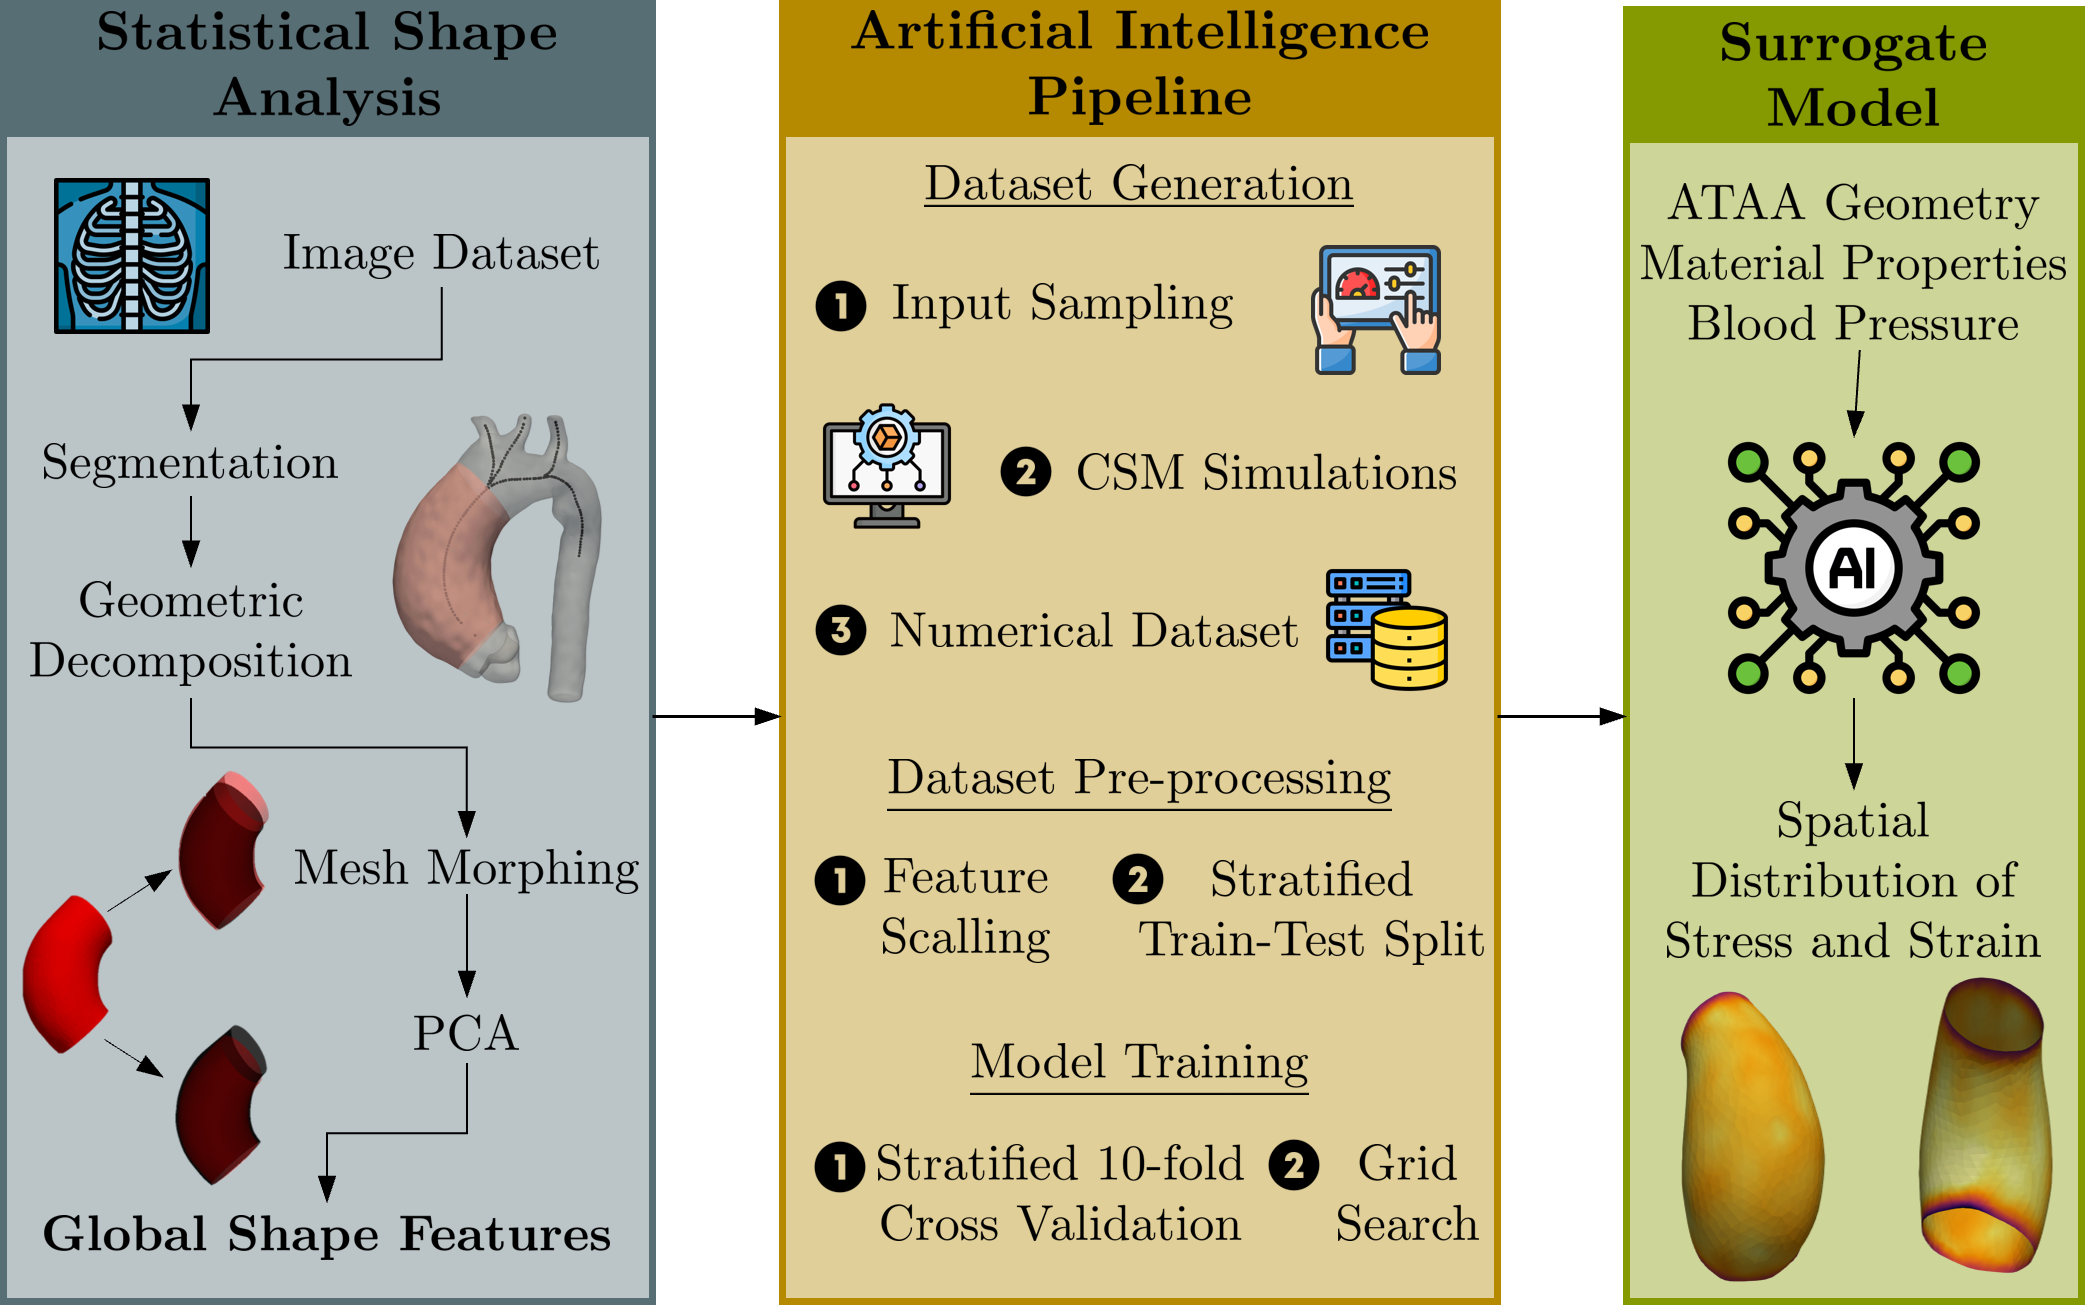
\includegraphics[width=0.95\textwidth]{fig1}
  \caption{Overview of the methodology employed to develop an AI-based surrogate model of~\gls{ATAA} wall mechanics. Statistical shape analysis was applied to an image dataset to extract global shape features via~\gls{PCA}. These features, combined with material properties and blood pressure, were used to generate a dataset of CSM simulations. The dataset was pre-processed and employed to train the surrogate model using stratified 10-fold cross-validation and grid search. The trained model predicts the spatial distribution of wall stress and strain.}
  \label{fig:workflow}
\end{figure}

\subsection{Patient-specific anatomy dataset}
  This work utilized patient-specific~\gls{CTA} data from 70 individuals diagnosed with~\glspl{ATAA}, comprising cases with both~\gls{BAV} and~\gls{TAV}. All patients were recruited under the scope of the AneurysmTool project (DOI: 10.54499/PTDC/EMD-EMD/1230/2021) and provided written informed consent. The study protocol was approved by the Ethics Committee of the \textit{Unidade Local de Saúde São José}.

  The~\gls{CTA} scans were acquired using a Revolution CT scanner (GE Healthcare, Milwaukee, WI, USA) with administration of an iodinated contrast agent (Ultravist 370, Bayer, Leverkusen, Germany), resulting in volumetric datasets of 512~$\times$~512~$\times$~292 voxels, with an isotropic spatial resolution of 0.63~\si{\milli\meter}. Aortic lumen segmentations were obtained at two phases of the cardiac cycle using a in-house build multi-view 2D U-Net. This method employs three independently trained U-Net encoder–decoder architectures, corresponding to the axial, coronal, and sagittal planes, in order to balance segmentation accuracy and computational efficiency. A total of $K=94$ segmentations were generated with at least one of each patient. Issues were found in some segmentations and excluded from the study.

  Following segmentation, the ascending aorta was geometrically isolated to focus the analysis on this region of interest. This was achieved by slicing the aortic lumen at the sinotubular junction and at the first ostium of the brachiocephalic artery. The extraction process relied on computing the aortic centerline using the inscribed sphere method and Voronoi diagram-based techniques.

\subsection{Mesh morphing}
  Developing a~\gls{SSM} of the~\gls{ATAA} requires generating a set of iso-topological meshes that represent patient-specific anatomies. This was accomplished through a two-step procedure. First, all segmented~\gls{ATAA} surfaces were spatially aligned with a reference mesh using an iterative closest point~(\gls{ICP}) algorithm to ensure consistent anatomical orientation. Second, the aligned reference mesh was deformed to fit each target surface using radial basis function mesh morphing. A thin plate spline kernel was selected to interpolate displacements across the 3D domain.

  A key challenge in morphing anatomical structures lies in the absence of distinct anatomical landmarks. To address this, we developed an automated approach for extracting pseudo-landmarks—referred to as~\glspl{SP} to guide the morphing process. These~\glspl{SP} were defined by uniformly sampling previously extracted centerline-based splines along the aortic wall. For each geometry, 16~\glspl{SP} were selected per spline across 10 cross-sectional planes.

  The initial reference mesh was chosen as the surface corresponding to the average~\gls{ATAA} diameter and centerline length across the dataset~\cite{Geronzi2023_dy,GRASSI2011112}. A triangular surface mesh was then generated using A triangular surface mesh was generated using the TetGen libraries within the SimVascular framework~\cite{updegrove2017}, comprising $n = 1354$ elements.

  To reduce mesh distortion and improve consistency across the dataset, a refined template was generated by averaging the initially morphed meshes. The entire morphing procedure was then repeated using this mean template as the new reference. This iterative refinement yielded a robust and consistent set of iso-topological meshes for all patient-specific geometries.

\subsection{Statistical shape analysis}
  A statistical shape analysis was conducted on the iso-topological surface meshes to identify global shape features of the~\gls{ATAA}.~\gls{PCA} was employed for this purpose, implemented in Python using the \textit{scikit-learn} library. The resulting low-dimensional representation enabled compact characterization of each patient-specific geometry and was later used as input for the surrogate model.

  The spatial coordinates of each mesh were vectorized by concatenating the $x$, $y$, and $z$ components of all $n$ mesh nodes, resulting in a data matrix of size $K \times 3n$. Prior to~\gls{PCA}, the matrix was standardized using the \textit{StandardScaler} function to ensure zero mean and unit variance for each coordinate dimension across the dataset.

  \gls{PCA} was then applied to extract the principal modes of geometric variation. The first six principal components, ranked by decreasing explained variance, were retained for further analysis. Together, these components accounted for around 90\% of the cumulative morphological variance in the geometries dataset. The corresponding modes describe major patterns of morphological variation in the~\gls{ATAA}, such as elongation, dilation, and asymmetry.

\subsection{Numerical simulations of aortic wall mechanics}
  The mechanical response of the~\gls{ATAA} wall throughout the cardiac cycle was simulated using~\gls{CSM} simulations. The primary objective was to estimate the spatial distributions of the Second Piola-Kirchhoff stress tensor, $\bm{S}$, and the Right Cauchy-Green strain tensor, $\bm{C}$, under physiological pressure loading. These quantities were later used as output targets for the surrogate model.

  The solid domain was generated by extruding the iso-topological surface meshes along the outward normal direction, assuming a uniform wall thickness. The resultant surface mesh of the~\gls{ATAA} wall was then meshed using the Gmsh library. A Python-based pipeline was developed to automate this step, ensuring consistent mesh generation across all patient-specific geometries. Node correspondence was preserved between the surface and volumetric meshes to maintain compatibility with the global shape features extracted through statistical shape analysis.

  The aortic wall was modelled as a homogeneous, isotropic, incompressible, Neo-Hookean material. A monolayer structure with constant wall thickness was assumed for all geometries. To better reflect physiological conditions, prestressing was included, following the method described by~\citet{hsu2011}. This approach estimates the prestress tensor required to balance the hemodynamic loads at the diastolic phase, thus estimating the intramural stress state of the aortic wall. As for boundary conditions, a homogeneous pressure load was applied to the luminal surface of the aortic wall. The pressure values followed an idealized curve. At the proximal and distal extremities of the domain, the displacements were fixed.

  All simulations were carried out using SimVascular on a workstation equipped with an Intel Xeon Gold 6242R 3.10 GHz CPU and 40 cores. A total of 4000 simulations were attempted, of which 3911 were successfully completed. The aortic wall density and Poisson's ratio were fixed at 1120~\si{\kilogram\per\metre\cubed}~\cite{pasta2013,Attaran2018} and 0.49~\cite{farzaneh2019,Baumler2020}, respectively. Computational settings, including the time step size and number of time steps, were kept constant across all simulations. The varying variables included the wall thickness and Young's modulus, sampled from uniform distributions $U(1, 2.5)$~\si{\milli\meter}~\cite{Mensel2014} and $U(1, 4)$~\si{\mega\pascal}~\cite{Duprey2010}, respectively. The diastolic and systolic pressures also varied and the followed normal distributions $N(80, 16)$~\si{\mmHg} and $N(120, 16)$~\si{\mmHg}, respectively.

  In addition to varying mechanical and loading parameters, 500~\gls{ATAA} geometries were synthetically generated by sampling the first six~\gls{PCA} modes. Each mode was sampled from a normal distribution with zero mean and variance equal to the corresponding eigenvalue of the~\gls{PCA} covariance matrix, enabling the creation of anatomically plausible yet diverse shapes for the simulation campaign.
  
  \begin{figure}
    \centering
    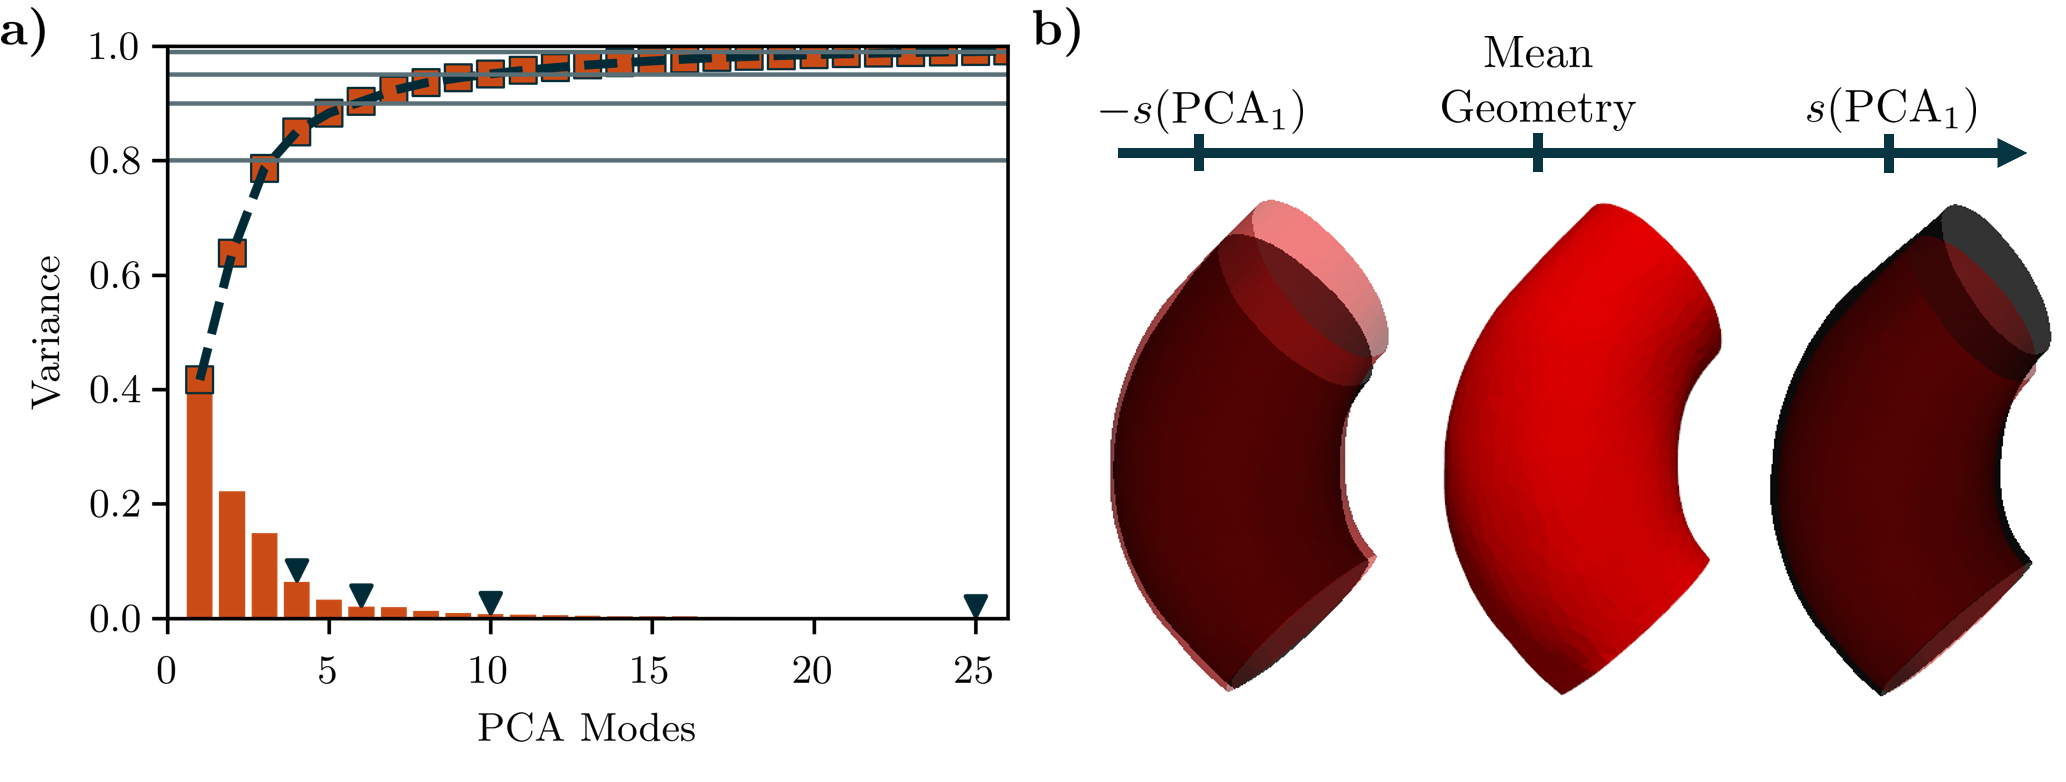
\includegraphics[width=0.95\textwidth]{fig2}
    \caption{Results of the~\gls{SSM}: a) compactness curve of the~\gls{PCA} (the symbols mark the number of modes required to capture 80 \%, 90 \%, 95 \%, and 99 \% of the cumulative variance), and b) geometric variations imposed by the first~\gls{PCA} mode on the mean shape (bright red).}
    \label{fig:pcaRes}
  \end{figure}

\subsection{Artificial intelligence pipeline}
  \subsubsection{Dataset generation}
    The dataset used to train the surrogate model was constructed from the results of the~\gls{CSM} simulations described previously. From each simulation, 20 samples were extracted, corresponding to 20 different loading states throughout the cardiac cycle. Each sample was defined by a unique combination of geometry, material properties, and loading conditions, resulting in a total of $m = 78220$ samples.

    Each data sample consisted of an input–output pair. The input vector contained 10 features: the first six corresponded to the first six~\gls{PCA} modes, representing the patient-specific geometry. The remaining four included wall thickness, Young's modulus, diastolic pressure, and the instantaneous pressure applied.

    The output vector captured the nodal distribution of two tensor fields: the Second Piola-Kirchhoff stress tensor, $\bm{S}$, and the Right Cauchy-Green strain tensor, $\bm{C}$. For each node in the iso-topological mesh, the six unique components of each tensor (due to symmetry) were recorded. As a result, each row of the output dataset had a length of $n \times 12$, with the first half corresponding to the components of $\bm{S}$ and the Second half to those of $\bm{C}$.

  \subsubsection{Data pre-processing}
    To improve the robustness of the training process and ensure balanced data distribution across training, validation and testing splits, a stratified sampling strategy was employed. Specifically, the dataset was clustered into clusters using the \textit{KMeans} algorithm, based on the input features. These clusters were then used to perform a stratified shuffle split via the \textit{StratifiedShuffleSplit} function from the \textit{scikit-learn} library. The data was divided into training (80\%) and testing (20\%) sets. Within the training set, an additional 10\% was reserved for validation, resulting in final proportions of 72\% for training, 8\% for validation, and 20\% for testing.

    All input features were standardized using the \textit{StandardScaler} from \textit{scikit-learn}, applied only to the training data to avoid data leakage. This process ensures that each feature has zero mean and unit variance. The scaling parameters computed from the training set were then used to transform both the validation and testing sets, maintaining consistency across the datasets. Additionally, this transformation was performed independently for groups of variables with the same order of magnitude, ensuring that each group was scaled to have zero mean and unit variance. For instance, the~\glspl{PCA} modes were scaled together, while the wall thickness, Young's modulus, and pressure values were scaled separately.
        
    \begin{figure}
      \centering
      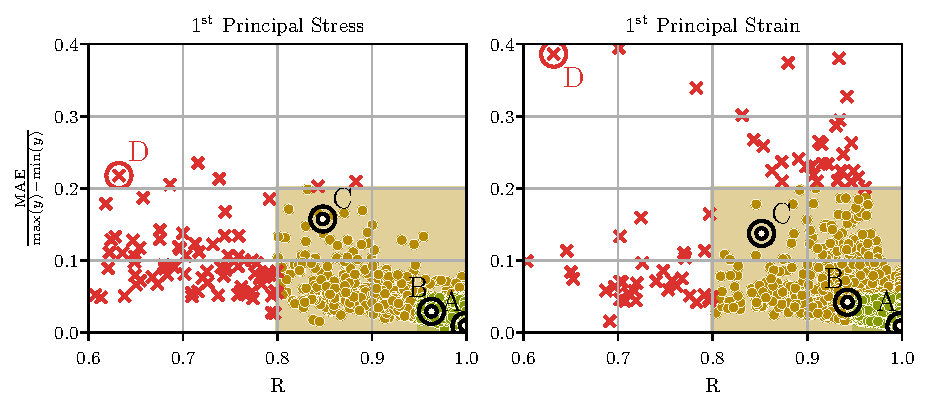
\includegraphics[width=0.95\textwidth]{fig3}
      \caption{\gls{DNN} performance overview: summary of the NMAE and R for all test samples.}
      \label{fig:performance_overview}
    \end{figure}

  \subsubsection{Model training}
    To perform regression operations, in particular when coupling~\gls{CSM} data and~\gls{ML}, neural networks are the most commonly used approach~\cite{phellan2021}. There are also known for being capable of handling nonlinear relationships between high-dimensional input and output data~\cite{Liang2018b}. This is particularly relevant, as the developed model aims to estimate the nodal distribution of the Second Piola-Kirchhoff stress and Right Cauchy-Green strain tensors. Also, this model was implemented using the \textit{PyTorch} framework.
    
    To identify the optimal set of hyperparameters, a grid search (\textit{GridSearchCV}) strategy was employed in combination with stratified 10-fold cross-validation (\textit{StratifiedKFold}). The grid search exhaustively evaluated combinations over a predefined parameter space, including learning rate, number of hidden layers, number of neurons per layer, dropout rate, and batch size. The final hyperparameters used for training are summarized in Table \ref{tab:final_hyperparams}. 
    
    \begin{figure}
      \centering
      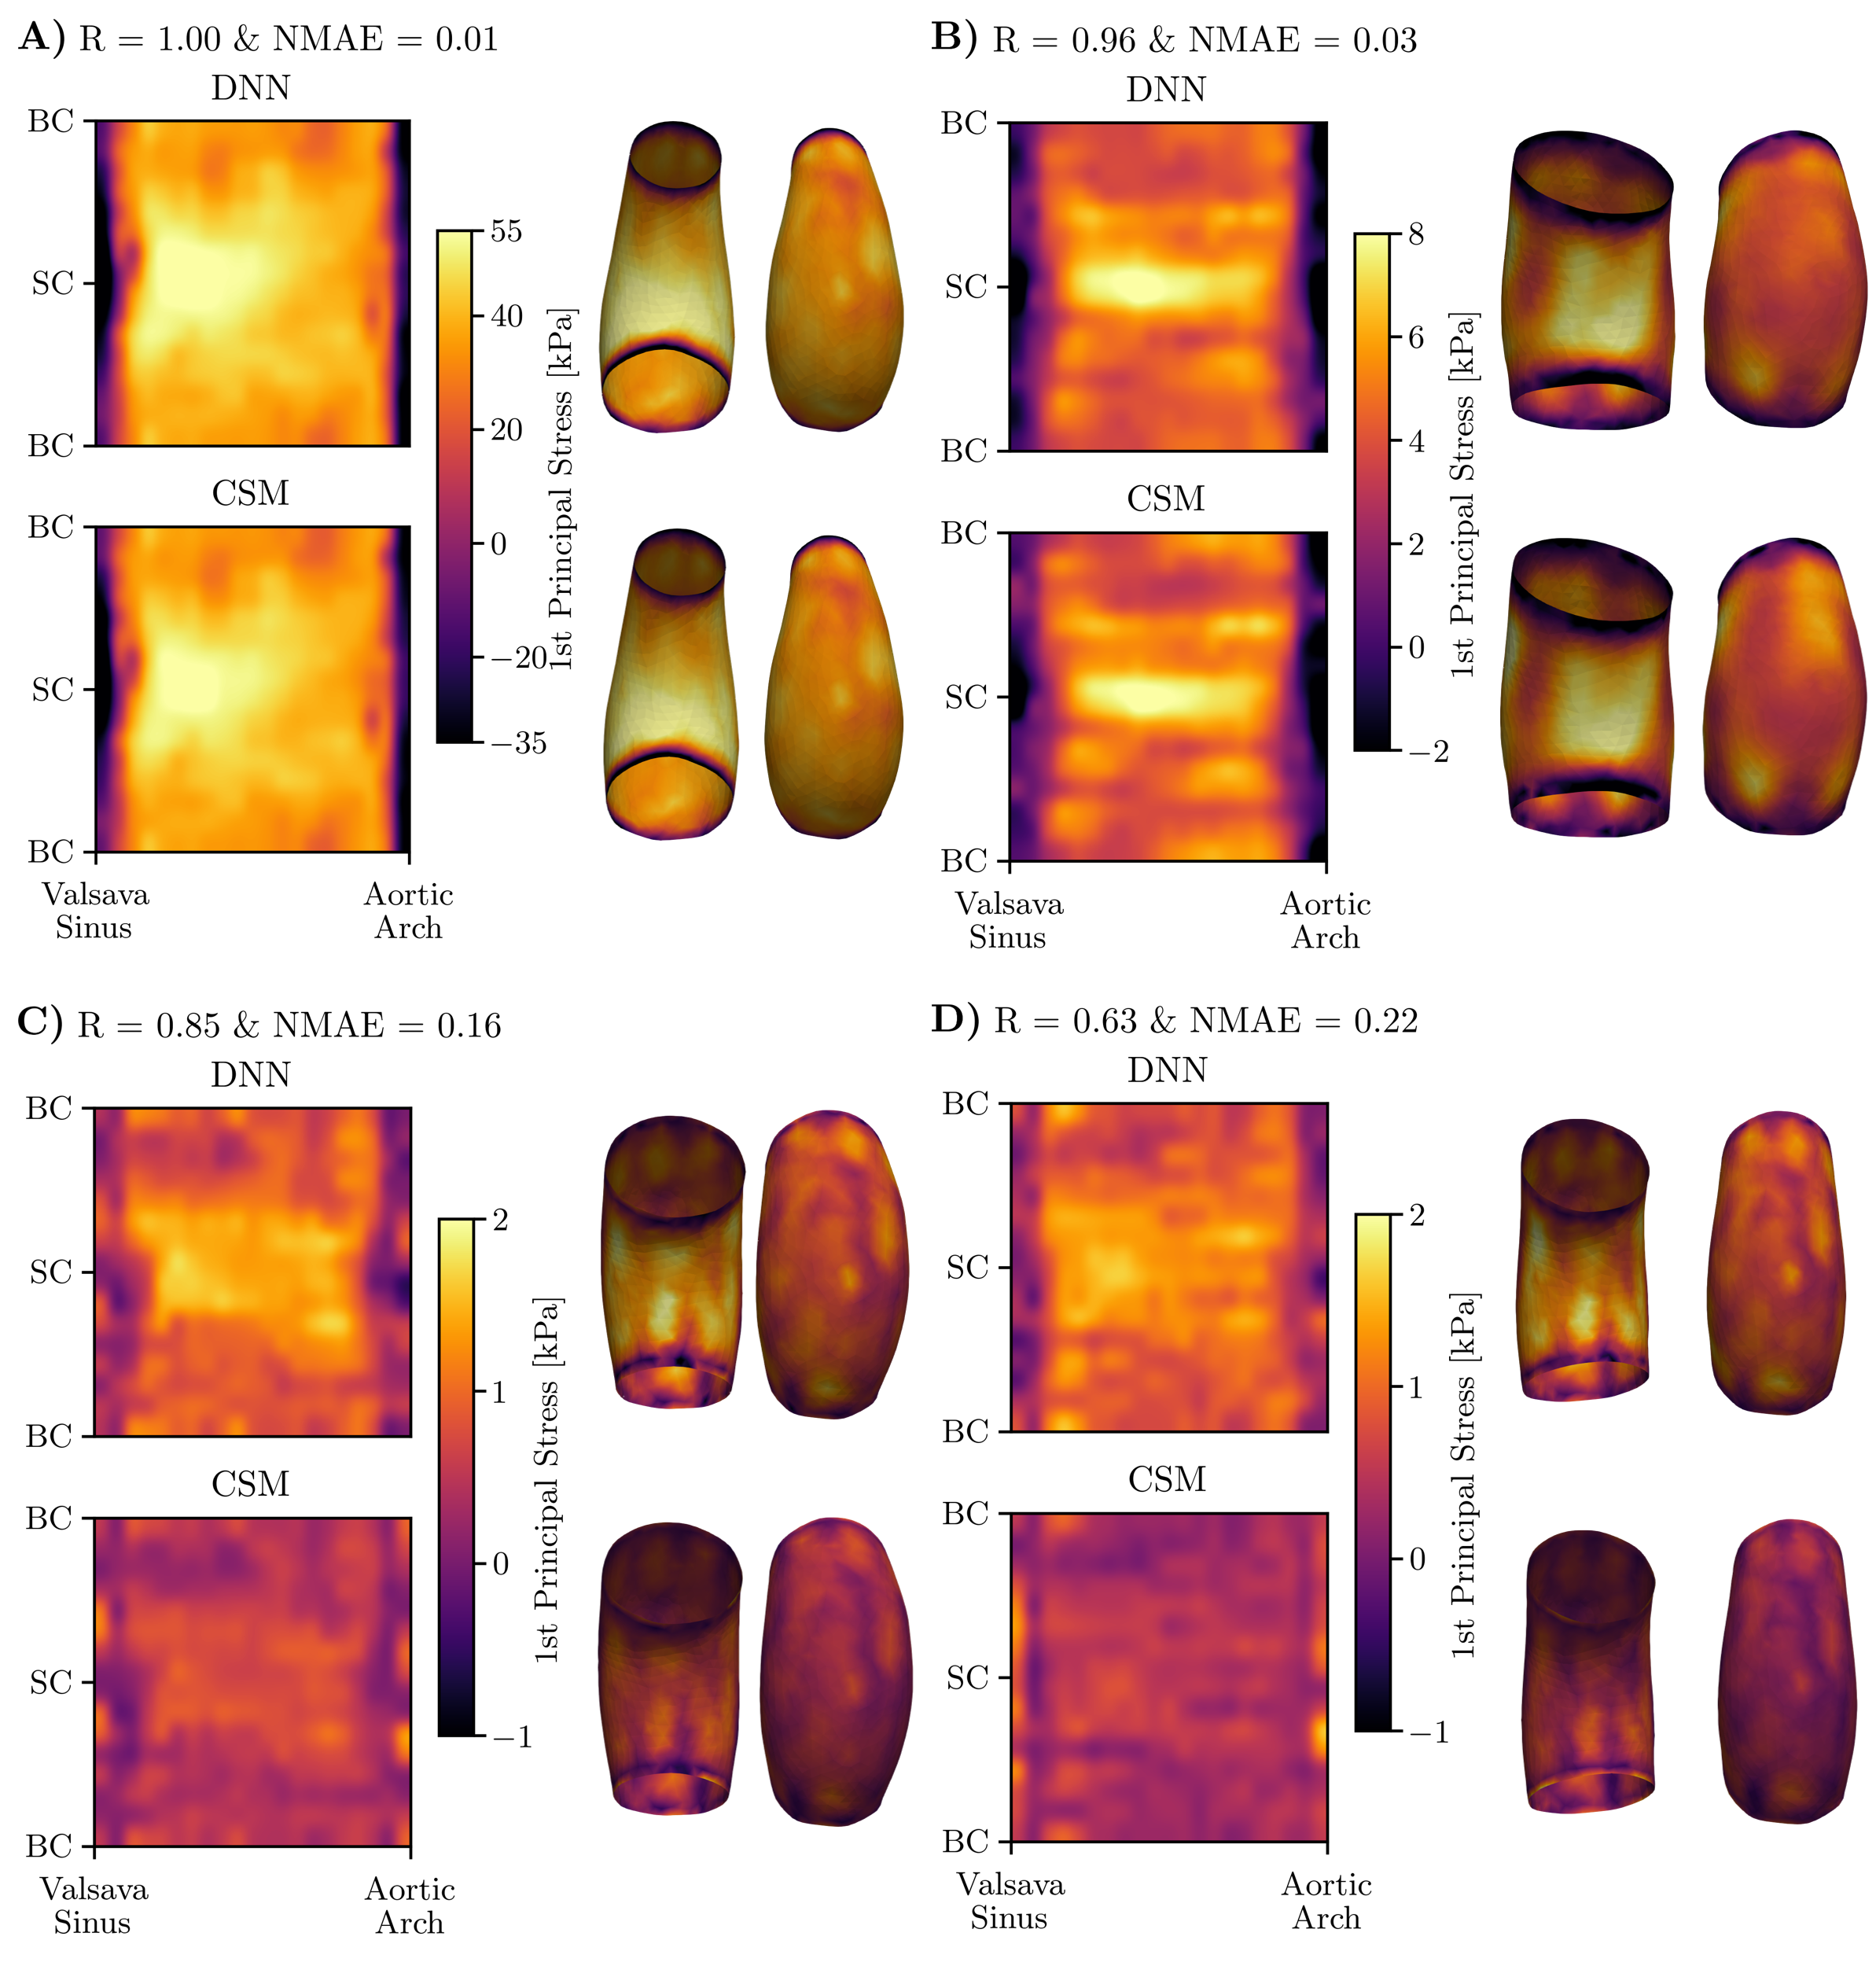
\includegraphics[width=0.9\textwidth]{fig4}
      \caption{Surface representation of the surrogate and~\gls{CSM} model predictions of the first principal stress.}
      \label{fig:surface_representationStress}
    \end{figure}    

    \begin{figure}
      \centering
      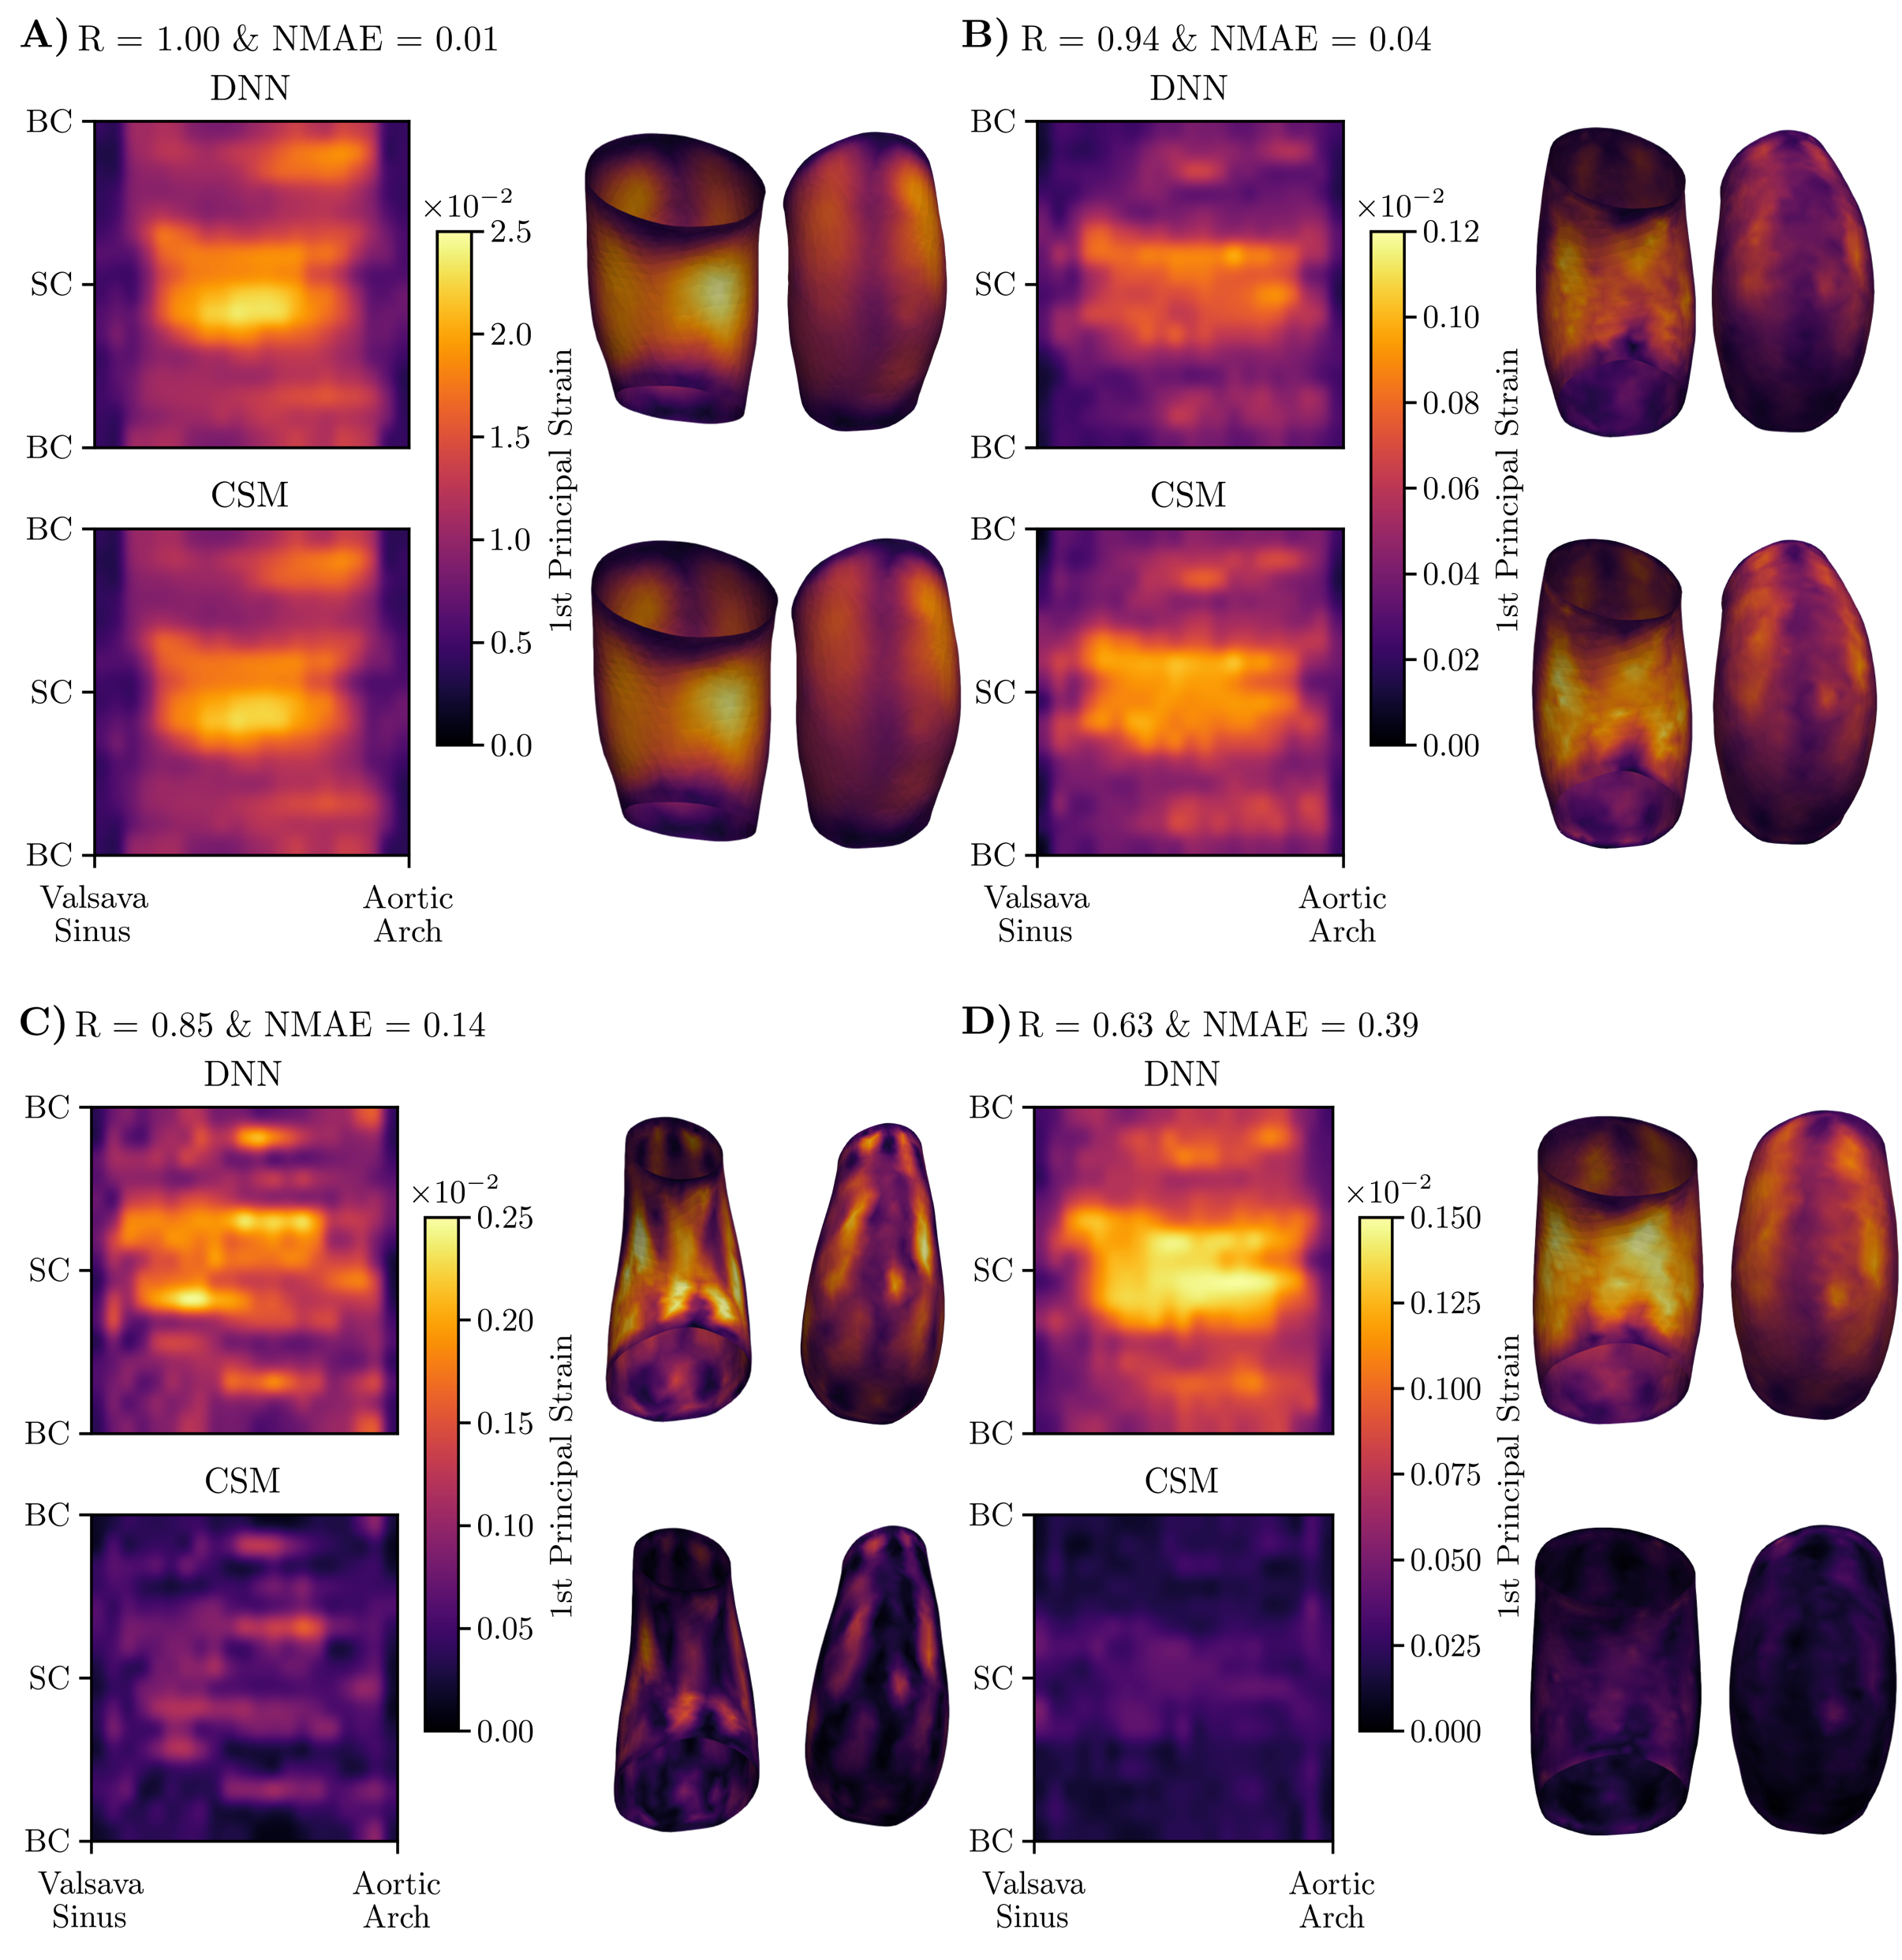
\includegraphics[width=0.9\textwidth]{fig5}
      \caption{Surface representation of the surrogate and~\gls{CSM} model predictions of the first principal strain.}
      \label{fig:surface_representationStrain}
    \end{figure}
      
    \begin{table}
    \centering
    \caption{Final hyperparameters used in the training of the surrogate model.}
    \label{tab:final_hyperparams}
    \begin{tabular}{@{}ll@{}}
    \toprule
    \textbf{Hyperparameter}     & \textbf{Value}          \\ \midrule
    Hidden layers           & 64, 128, 256, 512, 1024 \\
    Activation function         & ReLU                    \\
    Batch size                  & 400                     \\
    Optimizer                   & Adam                    \\
    Dropout rate                & 0.2                     \\
    Epochs                      & 152                     \\
    \bottomrule
    \end{tabular}
    \end{table}

    The loss function used during training was suggested by~\citet{Ghazi2021}, which aims to penalize more for elements with higher variation across the training samples. The loss function is as follows:

    \begin{equation}
      \mathrm{loss} = \frac{1}{n \times m} \sum_{i=1}^{n} \left( \sum_{j=1}^{m} s_i \left( y_i - \hat{y}_i \right)^2 \right)
    \end{equation}
    \noindent where $n$ is the number of nodes, $m$ is the number of samples, $s_i$ is the standard deviation of the $i$-th node across all samples, $y_i$ is the true value at the $i$-th node, and $\hat{y}_i$ is the predicted value at the same node.

  \subsubsection{Performance metrics}
    To evaluate the performance of the trained neural networks, two metrics were computed across all testing samples: the normalized mean absolute error, NMAE, and the Pearson correlation coefficient, R. The NMAE was computed as:

    \begin{equation}
      \mathrm{NMAE} = \frac{1}{m} \sum_{i=1}^{m} \frac{|y_i - \hat{y}_i|}{\max(y_i) - \min(y_i)}
    \end{equation}
      
    These metrics were estimated independently for the predicted distributions of Second Piola-Kirchhoff stress ($\boldsymbol{S}$) and Right Cauchy-Green strain ($\boldsymbol{C}$). Additionally, the same analysis was repeated for the subset of patient-specific~\gls{ATAA} geometries. To better access the performance of the surrogate model, two thresholds for success were defined:
    \begin{itemize}
        \item Moderate agreement: $\mathrm{R} > 0.8$ and $\mathrm{NMAE} < 0.2$
        \item High agreement: $\mathrm{R} > 0.95$ and $\mathrm{NMAE} < 0.05$
    \end{itemize}

% %%%%%%%%%%%%%%%%%%%%%%%%%%%%%%%%%%%%%%%%%%
% %%%%%%%%%%%%%%%%%%%%%%%%%%%%%%%%%%%%%%%%%%
\section{Results} \label{sec:results}
\begin{figure}
  \centering
  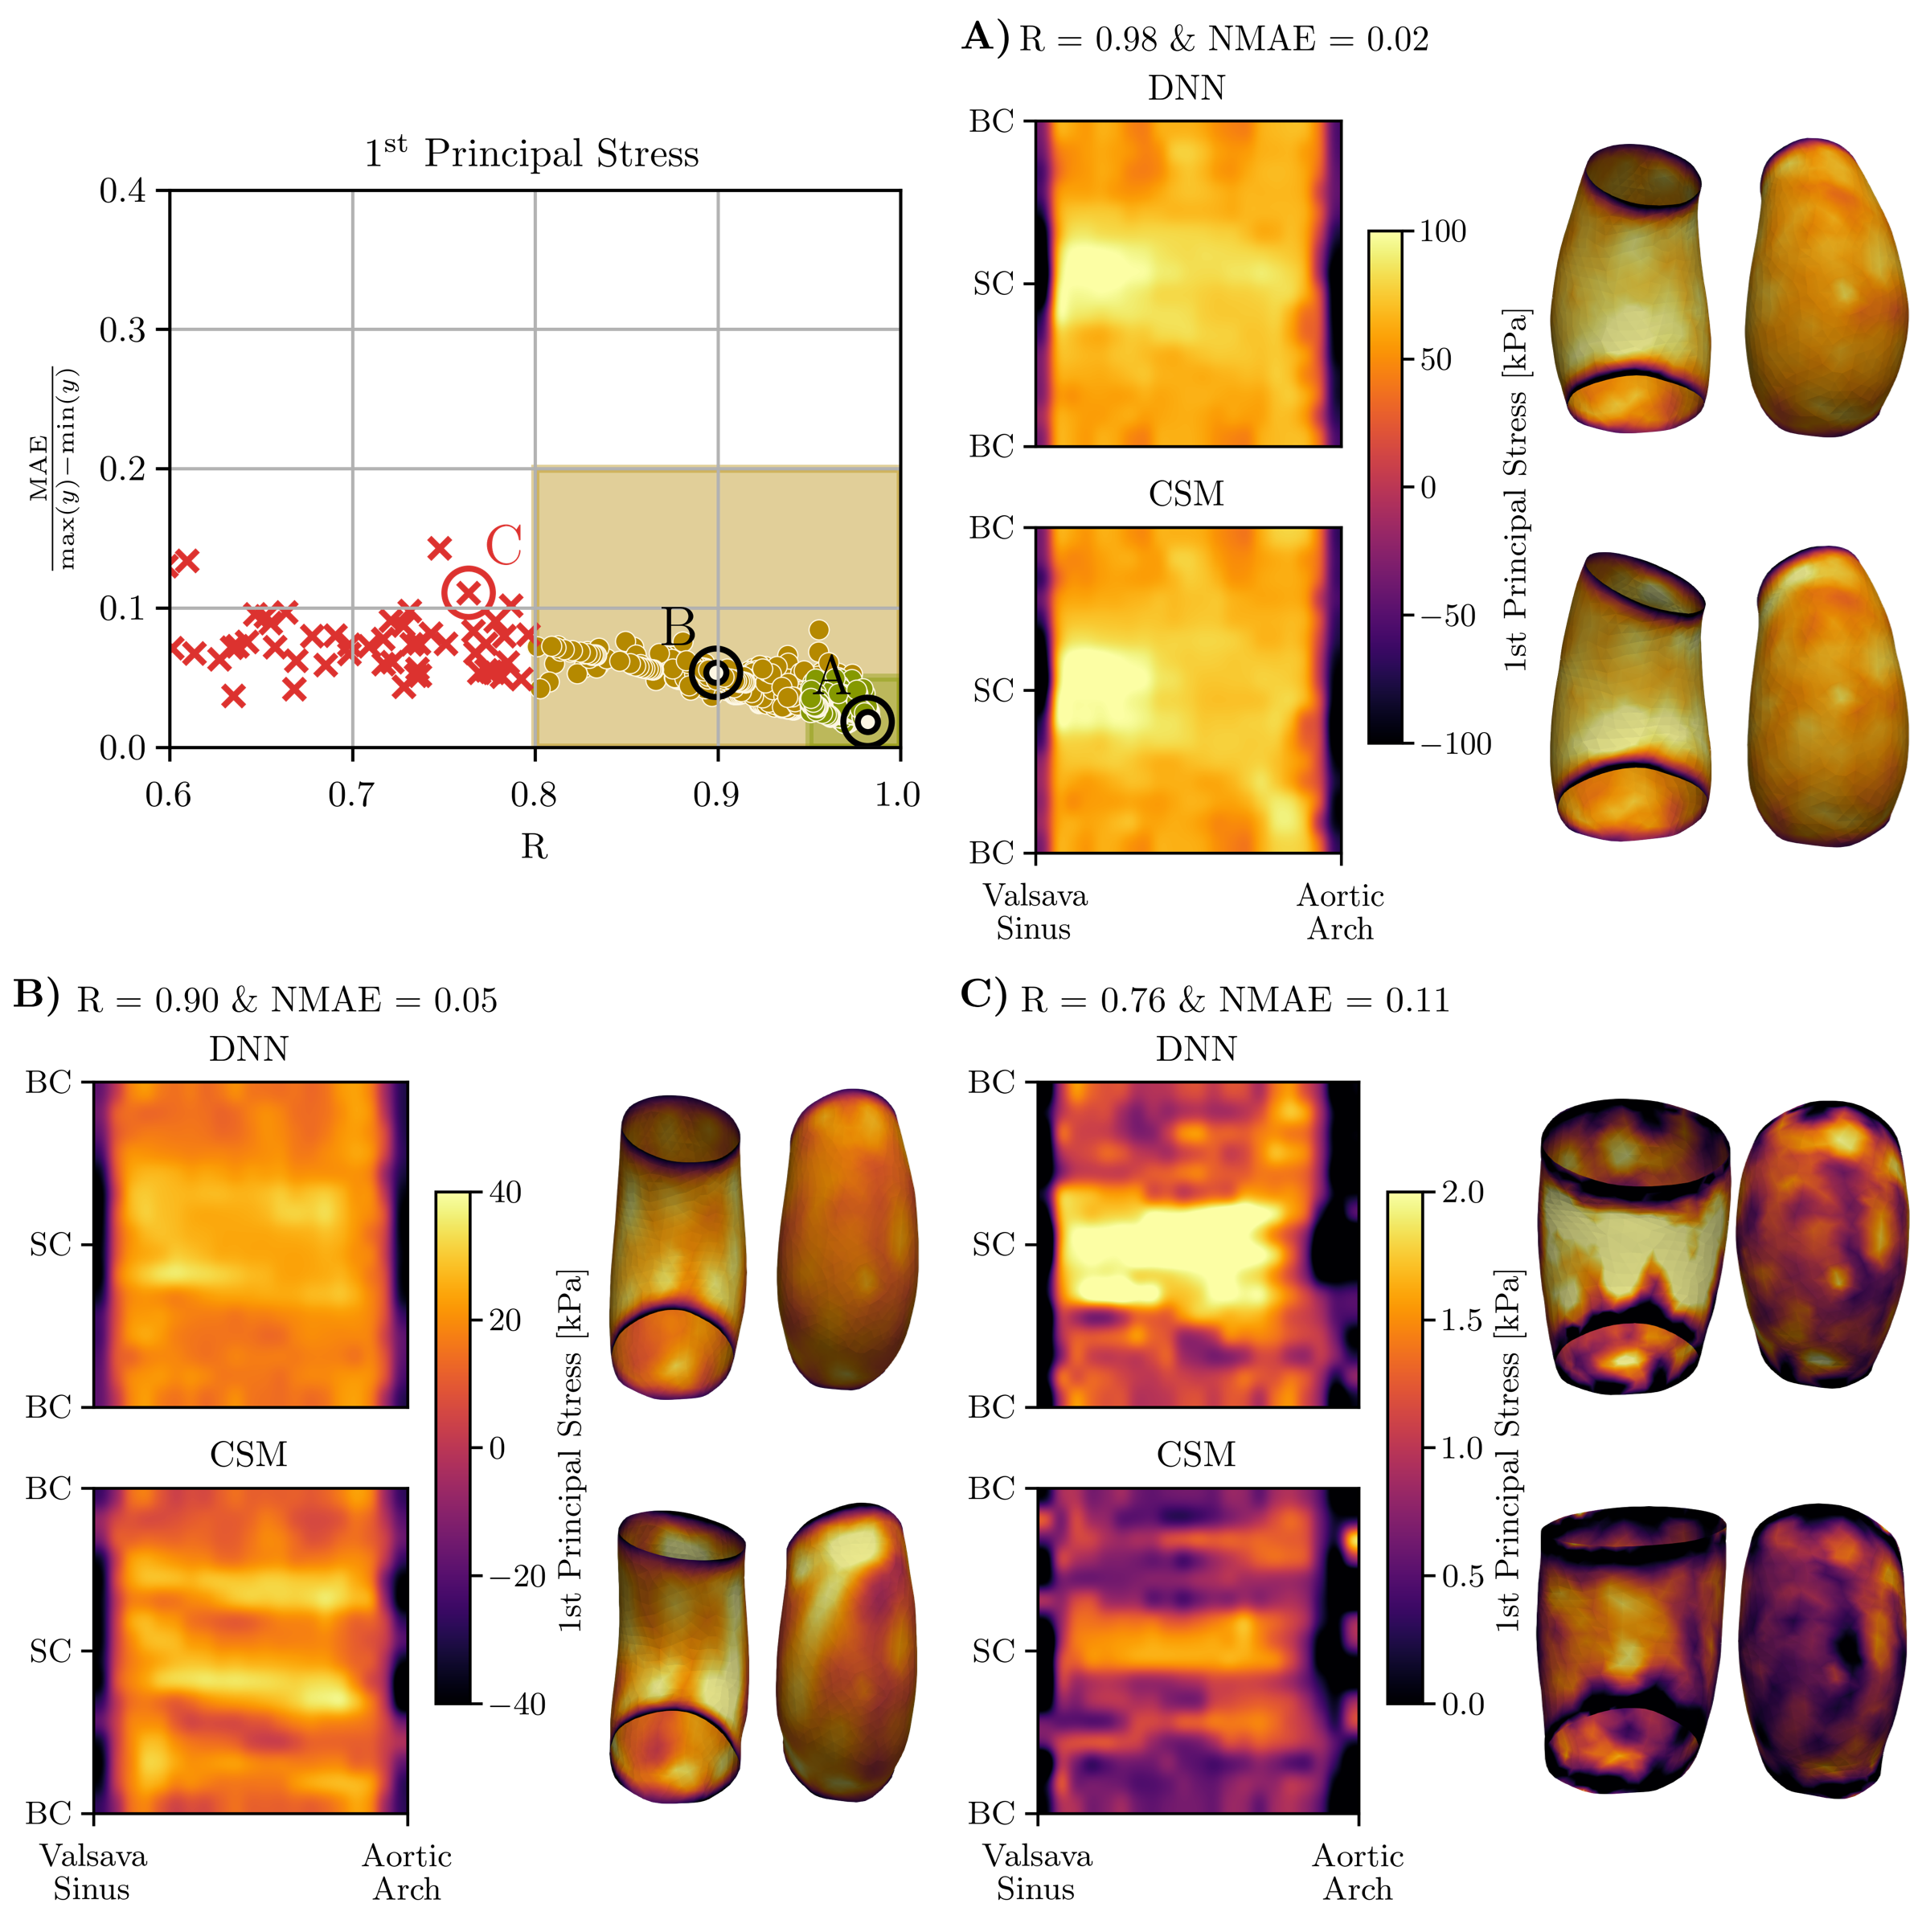
\includegraphics[width=0.9\textwidth]{fig6}
  \caption{Surface representation of the surrogate and~\gls{CSM} model predictions of the first principal stress for the patient-specific anatomy dataset.}
  \label{fig:surface_representationPSStress}
\end{figure}

\begin{figure}
  \centering
  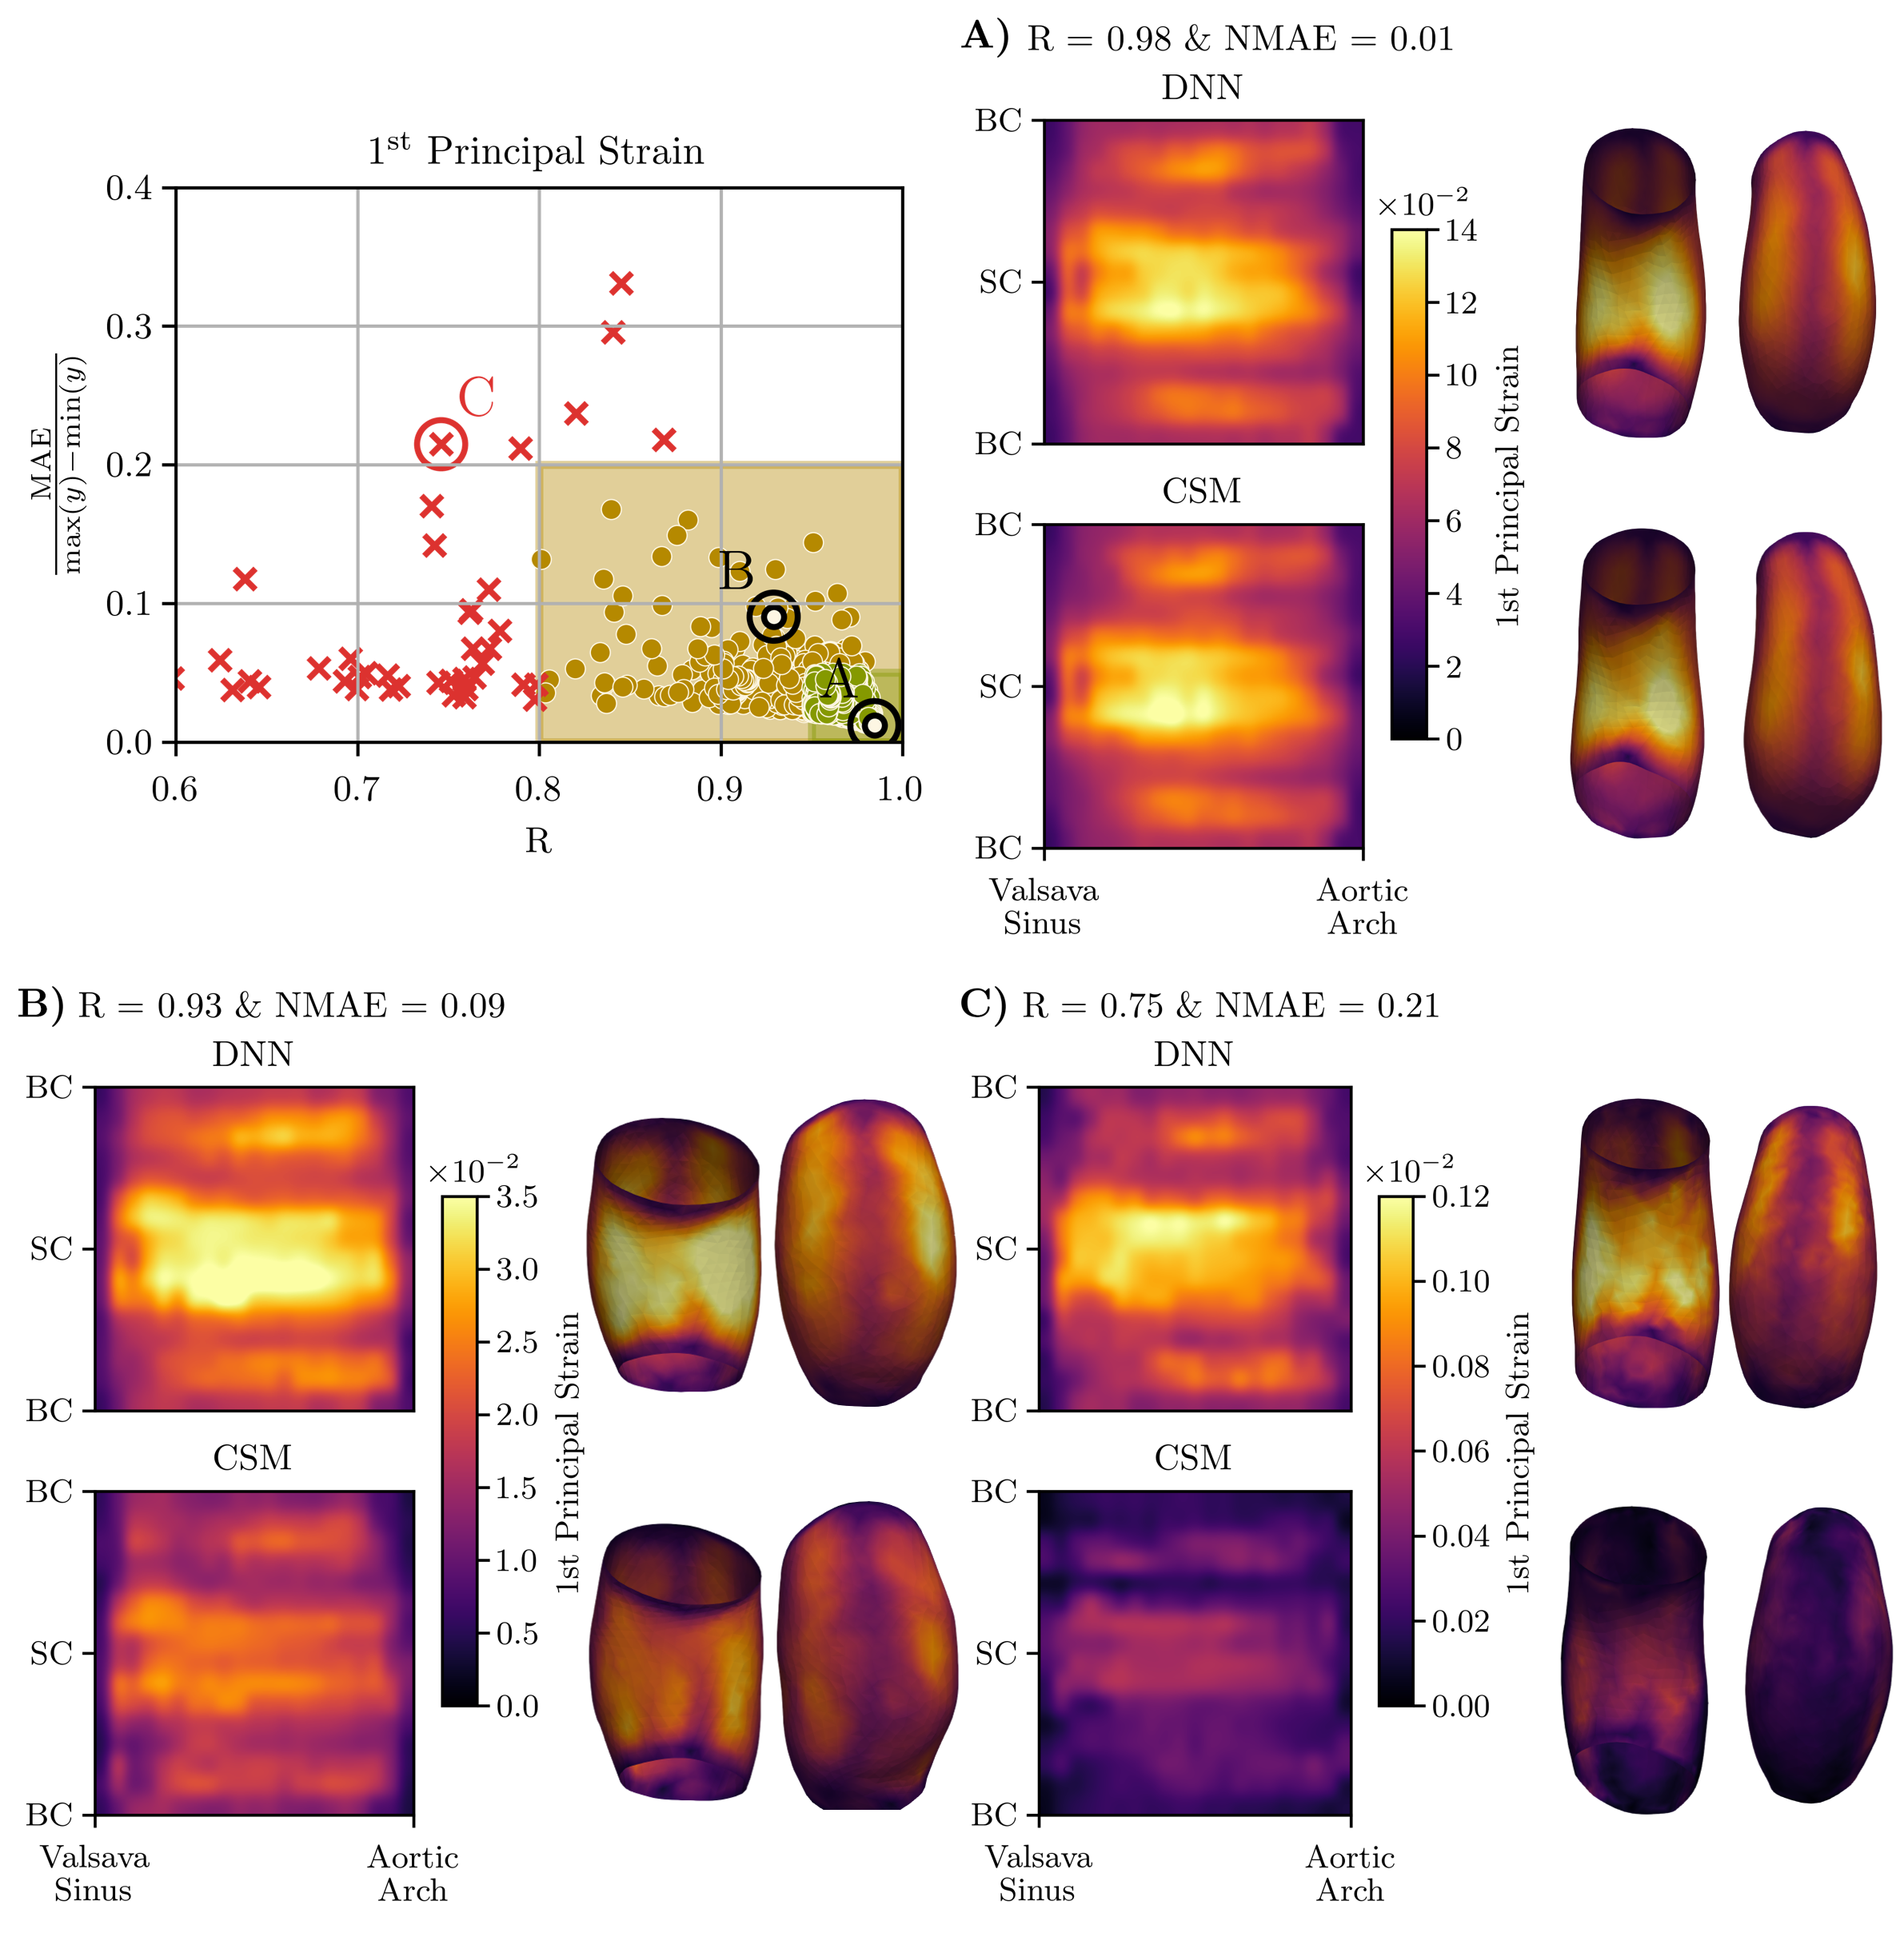
\includegraphics[width=0.9\textwidth]{fig7}
  \caption{Surface representation of the surrogate and~\gls{CSM} model predictions of the first principal strain for the patient-specific anatomy dataset.}
  \label{fig:surface_representationPSStrain}
\end{figure}

\subsection{PCA results}
  Concerning the results of the~\gls{SSM}, Fig. \ref{fig:pcaRes}-a shows the compactness curve. The first mode alone captures approximately 42 \% of the anatomical variation in the sample of patient-specific geometries characterized with iso-topological meshes. The Second and third modes represent 22 \% and 15 \%, respectively. Together, these three modes account for nearly 80 \% of the variability. The 90 \%, 95 \%, and 99 \% thresholds of the compactness curve were reached using 6, 10, and 25~\gls{PCA} modes, respectively. Fig. \ref{fig:pcaRes}-b illustrates the changes in geometry obtained by varying the first~\gls{PCA} mode around the mean shape.

\subsection{Neural network performance} 
  \subsubsection{Case 1 -- PCA driven geometries}
    Fig. \ref{fig:performance_overview} summarizes the NMAE and R of all test samples. For the predictions of the Second Piola-Kirchhoff stress tensor components, 99 \% and 96 \% of the samples showed a moderate and high agreement, respectively. For the predictions of the Right Green-Cauchy strain tensor, 99 \% and 95 \% of the samples fell into these categories, respectively.

    Fig. \ref{fig:surface_representationStress} and Fig. \ref{fig:surface_representationStrain} present the surface representations of the first principal stress and strain for four representative test cases. These examples cover different levels of agreement between the surrogate model predictions and the~\gls{CSM} simulations: A) very high, B) high, C) moderate, and D) low agreement. The heatmaps illustrate the spatial distribution in the ascending aorta mapped into a topologically equivalent rectangle. The $y$-axis corresponds to the circumferential direction, with BC and SC denoting the big and small curvatures, respectively, while the $x$-axis corresponds to the axial direction.
     
    For stress predictions, across all agreement levels the estimated and reference results exhibit similar spatial distributions. In particular, cases A and B also present a close match in magnitude. Cases C and D show an overestimation of stress magnitudes compared with the reference values. The predictions of the first principal strain follow the same trend, with the overestimation in cases C and D appearing even more pronounced.

  \subsubsection{Case 2 -- Patient-specific geometries}
    The performance of the surrogate model was also evaluated using the set of patient-specific anatomies employed in the~\gls{PCA} analysis. Figs. \ref{fig:surface_representationPSStress} and \ref{fig:surface_representationPSStrain} illustrate the comparison between surrogate model predictions and reference~\gls{CSM} results for the first principal stress and strain, respectively. These figures follow the same rationale as in Case 1, including both the performance overview and the surface representation analysis. 

    For the patient-specific geometry dataset, the success rates for high agreement changed notably: 51 \% and 64 \% for the predictions of the Second Piola-Kirchhoff stress and Right Green-Cauchy strain, respectively. Nonetheless, the success rates for moderate agreement remained similar (95 \% and 97 \%, respectively). As with the PCA-driven cases, the~\gls{DNN} predicted spatial distributions follow the same qualitative patterns as the~\gls{CSM} simulations. However, more pronounced differences in the magnitude of the variables are observed in regions of reduced mechanical loading.

\subsection{Correlation between error and inputs}
  Fig. \ref{fig:inVsout} examines how the prediction error of the surrogate model varies with different input parameters. The most noticeable trend is observed for the instantaneous pressure: as the pressure increases, the prediction error decreases significantly. For the remaining variables, including the PCA shape modes, wall thickness, and Young's modulus, no clear or consistent relationship with the error can be identified. 
  
  \begin{figure}
    \centering
    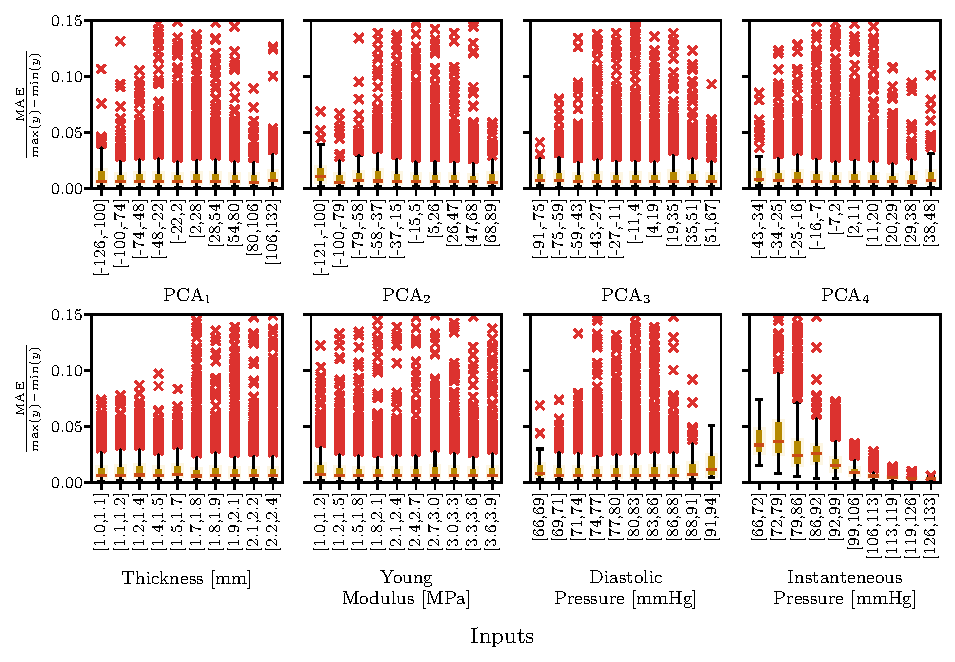
\includegraphics[width=.95\textwidth]{fig8}
    \caption{Correlation between the NMAE of the surrogate model predictions and the input parameters.}
    \label{fig:inVsout}
  \end{figure}

%%%%%%%%%%%%%%%%%%%%%%%%%%%%%%%%%%%%%%%%%%
%%%%%%%%%%%%%%%%%%%%%%%%%%%%%%%%%%%%%%%%%%
\section{Discussion} \label{sec:discussion}
The work presented in this chapter introduced a surrogate modeling framework for predicting the mechanical response of~\gls{ATAA}. By combining~\gls{SSM},~\gls{CSM} simulations, and~\glspl{DNN}, we developed a tool capable of reproducing the spatial distribution of the Second Piola-Kirchhoff and Right Cauchy-Green tensors with good agreement to reference simulations. The model showed robust generalization across the input space, with its main sensitivity being associated with the loading conditions. In particular, prediction accuracy improved at higher instantaneous pressures, indicating that the surrogate performs more reliably under high loading conditions, such as peak systolic pressure.

One of the most relevant outcomes of this study is the gain in reporting time. While the reference~\gls{CSM} simulations required between 20--60 minutes to complete on a high-performance workstation, the surrogate model generated results in less than one second on a low-end computer. This substantial reduction in computational demand highlights the clinical potential of such approaches, where time-efficient tools are essential. The computational burden is transferred almost entirely to the training stage, enabling rapid deployment once the model is trained. Nonetheless, a limitation of this strategy is the need for retraining whenever significant changes are introduced, such as new input features. Retraining the surrogate model may also require performing new simulations, for instance if boundary conditions are altered.

The performance analysis also revealed a decrease in success rate when the surrogate was applied to patient-specific anatomies, when compared to~\gls{PCA}-driven geometries. This reduction underscores the importance of expanding the input space to better capture anatomical variability. As future work, training the model with a higher number of PCA modes (for instance, the first 25 modes, which describe 99\% of the shape variability) may improve predictive performance for patient-specific cases. Although this study focused on the ascending aorta, the proposed methodology could be extended to the full aortic geometry. Achieving this goal will require the development of more efficient mesh morphing strategies, capable of handling the increased anatomical complexity.

Additional improvements can also be made in the constitutive description of the aortic wall. The present framework assumes a homogeneous wall with constant thickness and material properties. More physiologically realistic descriptions, such as spatially varying thickness, heterogeneous material properties, and histo-mechanical constitutive models, would better capture the underlying biomechanics. Incorporating these features, together with numerical validation, will be key steps towards building clinically reliable digital twins of aortic aneurysms. Future work may also include in training the effects of hypertension and hypotension.

%%%%%%%%%%%%%%%%%%%%%%%%%%%%%%%%%%%%%%%%%%
%%%%%%%%%%%%%%%%%%%%%%%%%%%%%%%%%%%%%%%%%%
\section{Conclusion} \label{sec:conclusion}
One of the main bottlenecks limiting the introduction of numerical modelsof~\gls{ATAA} biomechanics is the long computational time required for patient-specific analyses. Deep Learning architectures trained on numerical simulation data offer a promising approach to overcome this limitation, as demonstrated in the present work. In this chapter, a surrogate model of~\gls{ATAA} wall mechanics was proposed, combining a~\gls{SSM},~\gls{DNN}, and~\gls{CSM} simulations. The surrogate model was able to reproduce the spatial distributions of the Second Piola-Kirchhoff and Right Green-Cauchy tensors across almost the entire test dataset. For the patient-specific geometries, more than 95~\% of the predictions reached at least moderate agreement, confirming the robustness of the approach. Overall, this chapter demonstrates the feasibility and impact of using data-driven surrogate modeling to accelerate patient-specific biomechanical analyses, representing a significant step toward clinical translation.

\section*{Acknowledgments}
This research was funded by the Portuguese Foundation for Science and Technology (FCT,IP) under the projects: “Fluid-structure interaction for functional assessment of ascending aortic aneurysms: a biomechanical-based approach toward clinical practice” (AneurysmTool) DOI: 10.54499/PTDC/EMD-EMD/1230/2021; UNIDEMI: UIDB/00667/2020 and UIDP/00667/2020; A. Mourato Ph.D. grant DOI:10.54499/UI/BD/151212/2021, R. Valente Ph.D. grant 2022.12223.BD.

% Credits and references 
% To print the credit authorship contribution details
\printcredits

%% Loading bibliography style file
\bibliographystyle{model1-num-names}
%\bibliographystyle{cas-model2-names}

\bibliography{cas-refs}

\end{document}

